\documentclass[a4paper,11pt]{article}  % font size 11pt set here
\usepackage{graphicx} % graphicx is the package for figures
\usepackage[top=2cm,bottom=2cm,left=2cm,right=2cm]{geometry} % make the margins the right size
\usepackage{parskip} % parskip separates non-indented paragraphs by a blank line.
\usepackage[backend=biber, style=ieee]{biblatex} % bibliography and citation handler
\usepackage{hyperref} % better internal referencing
\usepackage[title]{appendix} % allows appendices
\usepackage{url} % fix url runoffs in bibliography
\usepackage{attrib} % allow quote attributions
\usepackage{subcaption} % allow subfigures
\usepackage{wrapfig} % wrap text around figures
\usepackage{mwe} % helps with grid subfigures or something like that
\usepackage{array} % multicolumns
\usepackage[english]{babel} % fix backwards quotations
\usepackage[autostyle, english = british]{csquotes} % fix backwards quotations
\MakeOuterQuote{"}

\addbibresource{dissertation.bib} % tell biblatex where our bibliography is

\setcounter{biburllcpenalty}{7000} % fix runoffs
\setcounter{biburlucpenalty}{8000} % fix runoffs

% Here's the paper's title and author details.
\title{Automated Toxicity in Brazilian Online Political Discourse}
\author{Kai Barber-Harris}
%\date{}   % Remove this line if you actually want to see the date

% Here is the actual beginning of the document
\begin{document}
	
	%=========================================================================================================
	% Title page
	%=========================================================================================================
	\maketitle
	\vspace{5cm}
	\begin{abstract}
		In the past two decades, social media and widely available internet access in developed countries has provided a new and powerful surface for malicious actors to influence discussions. Of particular note and vulnerability to these manipulations is online political discussion, which has the outreach and potential to swing elections with millions of users regularly logging in and engaging in these discussions worldwide. In this report, we extract a set of communities from a large dataset of Brazilian political discussion on X, formerly Twitter, spanning just over 6 months across the most recent presidential election cycle. We use these communities to inform an analysis of the link between increased bot activity and heightened toxicity in multiple communities, providing a valuable baseline for further investigations to take place upon. We also present evidence for the general participation of bots across the broadest range of discussion, further raising concern for the validity of online political discourse.
	\end{abstract}
	
	\vfill
	
	\begin{center}
		I certify that all material in this dissertation which is not my own work has been identified.
	\end{center}

	Signed: 
	
	\begin{figure}
		\hspace*{2cm} \includegraphics[width=0.3\linewidth]{signature}
		\label{fig:signature}
	\end{figure}
	
	\newpage
	
	\tableofcontents
	
	\newpage
	%=========================================================================================================
	% Content starts here
	%=========================================================================================================
	\section{Introduction}
	\label{sec:intro}

	\subsection{Background and motivation}
	\label{subsec:background}
	In the past two decades, the rise of social media has led the world to become increasingly interconnected, with avenues for discussion of daily news, hobbies, music, and politics often no further away than the smartphones in our pockets. One of the most relevant social media platforms for this form of interpersonal discussion is X, formerly known as Twitter. X is a microblogging service designed to share short-form statements or questions and quickly spread these posts and ideas via the engagement of other users amplifying the post themselves. While not necessarily the most popular social media site\parencite{BiggestSocialMedia}, X's post format and engagement options often make it the platform of choice for users seeking discussion along with leaders and figureheads - or at least their public relations teams - wishing to more directly engage with their audience.
	
	More recently, major political events around the world point towards a more divided society than ever before, with election and major referendum results often coming down to the wire (\textcite{EUReferendumResults}, \textcite{FederalElections2016a}, \textcite{FederalElections2020a}, \textcite{SIGEleicaoResultados}). With this polarisation only becoming more pronounced over time, alongside the paradigm shift of political discourse and news dissemination more often taking place online especially with younger people\parencite{shearerSocialMediaOutpaces}, it is now common for voters to be loosely or even distinctly aware of the possibility of bad actors attempting to influence the zeitgeist of these discussions. A common fear is the use of automated actors, or "bots", continually posting opinionated messages or simply strengthening another account's postings to do this. Elon Musk, current CEO and owner of X, more than once attempted to use this very concern of bot presence to back out of his deal to buy the platform, including it as  evidence for a countersuit against X's board \parencite{MuskPublicVersion}\parencite{elonmusk[@elonmusk]Teslarati20Fake2022} who at the time were forcing Musk to follow through on the signed deal. 

	The potential payout for such manipulations is extremely high. For example, with Brazil being the 6th-largest audience for X boasting 22 million unique monthly users\parencite{TwitterGlobalAudience}, convincing some of these users to vote a specific way has the potential to sway elections - the most recent Brazilian presidential election was only won by a margin of approximately 6 million votes\parencite{SIGEleicaoResultados}. Further, the only cost to running these bots is that of some computation time and the development of their code - creating accounts on X is free\footnote{In the closing days of editing this report, Musk announced plans to charge newly-created accounts for the ability to post to the platform\parencite{espositoElonMuskConfirms2024}. However, it is unclear how exactly this will prevent bot accounts from being created in advance of their usage, and groups with sufficient funding (such as wealthy governments) can simply pay the price of entry.}. For any group seeking to influence political discourse or even entire elections, there are very few if any more cost-effective ways to go about it. This is evidenced by the interference of Russian groups in the 2016 US presidential elections via X, who appear to have used bots to amplify the messaging of manually operated accounts - most of which were "mostly promoting conservative causes and were, specifically, spreading pro-Trump material."\parencite{badawyAnalyzingDigitalTraces2018}
	
	It is for all of these reasons that we present the following work; we hope to further investigate automated posts concerning Brazilian politics on X with a specific focus on the trends of toxicity between different discussions, topics, and communities. While proving a link between any two of political leaning, bot postings, and average toxicity is unlikely, we hope that the exploration of such a subject may provide a more nuanced view on how these automated accounts may attempt to influence online political discourse in the modern day.

	\subsection{Specification}
	\label{subsec:spec}
	This project was undertaken with the overall goal of further investigating a pair of questions put forward in November 2023 as part of the related literature review:
	\begin{enumerate}
		\item Are bots performing in a coordinated manner attempting to influence political discussions to be more incendiary?
		\item Do coordinated activities or bot accounts admit a notable difference in average sentiment or stance toward a specific topic when compared to the generic real user base?
	\end{enumerate}
	The literature review also notes:
	\begin{quote}
		We would consider this project to be successful if either one of the two questions presented has been definitively answered, or both questions have been explored and further areas of research have been identified to expand upon the findings. A definitive answer to both questions would be considered to be an outstanding success.
	\end{quote}
	These questions and criteria provide us a strong framework with which to continue our report, in which we more so aim to explore these questions rather than answer them outright. However, due to a misunderstanding of the work, the sentiment and stance analysis was abandoned partway through the project (\autoref{subsec:sentiment}); as such, we cannot directly answer the second question posed, though we can instead adapt it:

		\quad \textit{Do coordinated activities or bot accounts admit a notable difference in average toxicity in different communities when compared to the generic real user base?}

	This adapted question is one we can make an attempt to answer within the scope of the work completed.
	\section{Data}
	\label{sec:data}
	\subsection{Overview}
	\label{subsec:overview}
	The data used for the project was provided by Diogo Pacheco, who advised on this work and has extensive experience in the field (\textcite{pachecoBotsElectionsControversies2023}, \textcite{pachecoUncoveringCoordinatedNetworks2021}, \textcite{chenNeutralBotsProbe2021},
	\textcite{pachecoUnveilingCoordinatedGroups2020}). The dataset in total comprises 437 million X posts made by 13 million unique users between August 2018 and March 2023. These posts are stored in a raw JSON format. A wealth of metadata about each individual post is also recorded alongside its original text in these JSON files. The data is recorded in files each containing a day of data each, and are labelled appropriately. 
	Pacheco also provided a set of PKL\footnote{PKL, or "pickle": Python-exclusive binary file type used to contain arbitrary data. Extremely efficient in storage space, but can only be effectively "unpickled" by a Python script.} files he had used in his own work previously, these files containing a preprocessed version of most (but not all) of the raw JSON files. Not all days with a JSON file have a corresponding PKL file, and vice versa.
	\subsection{Collection terms}
	\label{subsec:terms}
	The data was collected via the Twitter Streaming API before its shutdown in March 2023. The dataset contains posts collected from a set of keywords themed around Brazilian political discourse, chosen by Pacheco at the beginning of the collection period.
	
	Posts were also collected directly from candidate accounts, from posts containing the full name of any candidate, and from posts containing the official hashtag of each candidate's campaign. In July 2022, the collection was adjusted to include posts made by official party accounts; this is the only time the collection terms changed across the 5 years.
	
	\section{Algorithm Design}
	\label{sec:design}
	\subsection{Basic data filtering}
	\label{subsec:filters}
	Some caveats apply to the data that was carried through to the final analysis. As the provided JSON files do not contain a botscore for each post, and the PKL files do not contain the original text of the post, we are limited to only using days which have files of both types due to the nature of our analysis. Further, the sheer size of the dataset requires us to thin the data in order to perform meaningful analysis within a reasonable time frame (see \autoref{subsec:toxicity}). We chose at this point to work with the data beginning July 2022 and ending March 2023, after the single collection term adjustment. This range of dates contains 122 total days with corresponding PKL and JSON files, representing a total of 86,787,095 posts for analysis; approximately 20\% of the entire available dataset. 
	
	At this point we removed posts that contained no hashtags at all, along with all reposts. Posts without hashtags are irrelevant for our analysis, and a repost is a special posting action common on X. Reposts effectively share the original content of the post again to the reposter's followers. As these reposts are exact copies of the original, they can be safely removed for the purposes of our analysis. We elected to keep quoted posts, which are actions similar to reposts but which allow the reposting account to add their own unique comment alongside the original text. This quoted post can then itself be reposted or quoted. These quote posts were kept as the extra comment may include other hashtags the author has added, thereby making the post relevant for our analysis.

	\subsection{Collocations}
	\label{subsec:collocation}
	The planned analysis of hashtags and their attributes called for the construction of a collocation network. The algorithm for this work is fairly simple, and naturally involves filtering the dataset to a smaller size. First, we must take each post with 2 or more hashtags in it; this is easily accomplished as the PKL files contain the hashtags within each tweet. We can then sort the hashtags (to prevent reversed instances of the same pairs) and generate the pairwise combinations possible from the list of hashtags for each post.
	
	Recording the number of occurrences of these pairwise combinations constructs a collocation matrix; at the same time, we can track the number of times each hashtag appears in total to a separate "appearances" matrix. Respectively, these matrices act as edge and node tables, with the appearances of each collocation representing an edge weight and the appearances of each hashtag supporting a deeper analysis. For those unfamiliar with the terminology of graph theory, please refer to \autoref{app:networks}.

	\subsection{Modularity}
	\label{subsec:modularity}
	These edge and node tables can then be loaded into a network analysis program such as Gephi\parencite{GephiOpenGraph}. Using Gephi, we can inspect and analyse the data we have already found. In order to increase the clarity of investigation, at this time we chose to filter out all hashtags (and therefore their collocations) which appeared less than 1,000 times in total. This reduces the size of the network from 134,633 to 1,943 unique hashtags, a 98.5\% reduction. This same action also reduces the number of edges from 1,065,768 to 153,444, an 85.6\% reduction. With only 1.5\% of original nodes visible, nearly 15\% of original edges are still visible; these observations together show us that the most important nodes have by far the most connections with one another, and these "smaller" nodes can be filtered out safely. 
	
	The filter increases the relative "importance" of each node by removing smaller nodes which dilute the analysis; we can now be sure that each and every one of these hashtags is discussed in a significant manner. It should be especially noted that filtering out hashtags which appear less than 100 times across these 122 days results in a 93\% reduction in nodes, further proving that the vast majority of hashtags are not especially relevant to everyday discussion in online Brazilian political discourse and can safely be ignored for our analysis.
	
	With this filtering complete, we can run a modularity analysis on the graph with Gephi. Modularity analysis is a methodology for detecting communities in graphs with weighted edges. Gephi implements the Louvain-style modularity analysis, which finds communities by recursively taking the aggregate result of a smaller community-detection function \parencite{Findcommunities}. The result of this process is that each hashtag node will have a modularity class assigned to it, denoting the community it primarily belongs to. For our hashtag network, the Louvain analysis found 18 unique communities.

	\subsection{Toxicity}
	\label{subsec:toxicity}
	We now calculate the probability that any given post made in a hashtag would be considered toxic.
	The computation of the toxicity score for each hashtag follows an involved process. The steps are as follows:
	\begin{enumerate}
		\item Collect all hashtags which belong to the two largest modularity classes of left-wing and right-wing discussion (see \autoref{subsec:computation} for reasoning).
		\item \label{step2}For these hashtags, collect all posts in which any of these hashtags appear. In total, there were 968,627 of these posts.
		\item Preprocess the original text of each collected post through a standard natural language processing pipeline (tokenisation, lowercasing, removal of punctuation and stopwords, stemming).
		\item Run each preprocessed text through a pre-trained machine learning model to determine whether the post is toxic or not.
		\item For each hashtag, collect all posts containing that hashtag and calculate the mean toxicity of the posts. This score is then a floating point representing the likelihood of a post containing the hashtag to be toxic.
	\end{enumerate}
	The pre-trained machine learning model used was ToLD-Br, a "pre-trained Multilingual BERT fine-tuned with ToLD-Br" \parencite{leiteToxicLanguageDetection2020}. ToLD-Br is provided as open-source under the Creative Commons BY-SA 4.0 license, and as such allows us to use a previous work to greatly accelerate our own. The trained BERT model is a CUDA-accelerated\footnote{CUDA: NVIDIA owned and maintained framework for offloading repetitive, simple matrix and arithmetic operations to an attached graphics processing unit which excels at such tasks rather than the central processing unit of the computer, which is comparatively much worse at such operations.} binary classification transformer model which, given a text to process, outputs either a "toxic" or "non-toxic" interpretation. The model itself was trained on a dataset of Brazilian Portuguese X posts; this fits our use case perfectly, and we thank \citeauthor{leiteToxicLanguageDetection2020} for the model's contribution to the project.
	
	\subsection{Botscore}
	\label{subsec:botscore}
	Finally, we calculate the probability that any post made containing a given hashtag was posted by a suspected bot, or the mean "botscore" of the hashtag.
	Botscores for most posts in the dataset were already precalculated by the Botometer tool \parencite{sayyadiharikandehDetectionNovelSocial2020} within PKL files. As such, we can simply follow the final step of the toxicity calculation process, collecting the botscores for each post containing a given hashtag and calculating their mean to give an average botscore for this hashtag.

	These botscores are extremely valuable when taken in the context of X's recent history. Due to the acquisition and major changes to X since Elon Musk's takeover in late 2022, many useful tools for analysis have been taken offline due to sharp API cost increases and functionality changes. One of these casualties was Botometer, which was used to generate these botscores during Pacheco's earlier work \parencite{pachecoBotsElectionsControversies2023}. Botometer today still exists as "Botometer X", but it is severely hampered by these API changes.

	\section{Results and Analysis}
	\label{sec:results}
	\subsection{Hashtag Network}
	\label{subsec:network}

	At this time, the data processing is complete and we can begin our analysis. \hyperref[fig:1]{Figure 1} shows the fully filtered network after running the ForceAtlas 2 layout algorithm to convergence, with each node colour-coded to its modularity class\footnote{For the sake of presentation, the graph was also run through an algorithm preventing nodes from overlapping.}. ForceAtlas 2 is an continuous layout algorithm that works by repulsing all nodes from one another while attracting nodes based on edges\parencite{jacomyForceAtlas2ContinuousGraph2014}, but this work could easily be recreated with any suitable force-directed layout algorithm. In this graph, we can very clearly see the different communities present in our data, noting the presence of 4 "primary" communities\footnote{For more, see \autoref{app:modularities}}, shown in \autoref{tab:1}.

	The size of each hashtag is directly taken from the its number of appearances. We can easily identify central hashtags that appear often in their communities; the largest right-wing hashtag is "bolsonaro22", the official campaign hashtag for Jair Bolsonaro. Likewise, the largest left-wing hashtag is "lula13", Lula da Silva's official campaign hashtag. The largest battleground hashtags are those that are relevant to both of the previous communities; terms such as "eleicoes22" (election22), "brasil", and "riodejaneiro", all of which are topics and conversations that both left-wing and right-wing communities are likely to take part in - this is the essence of what makes a hashtag a "battleground". News hashtags include "globonews" (popular Brazilian news network), "nytimes", and "blacklivesmatter".

	\begin{figure}%[ht]
		\centering
		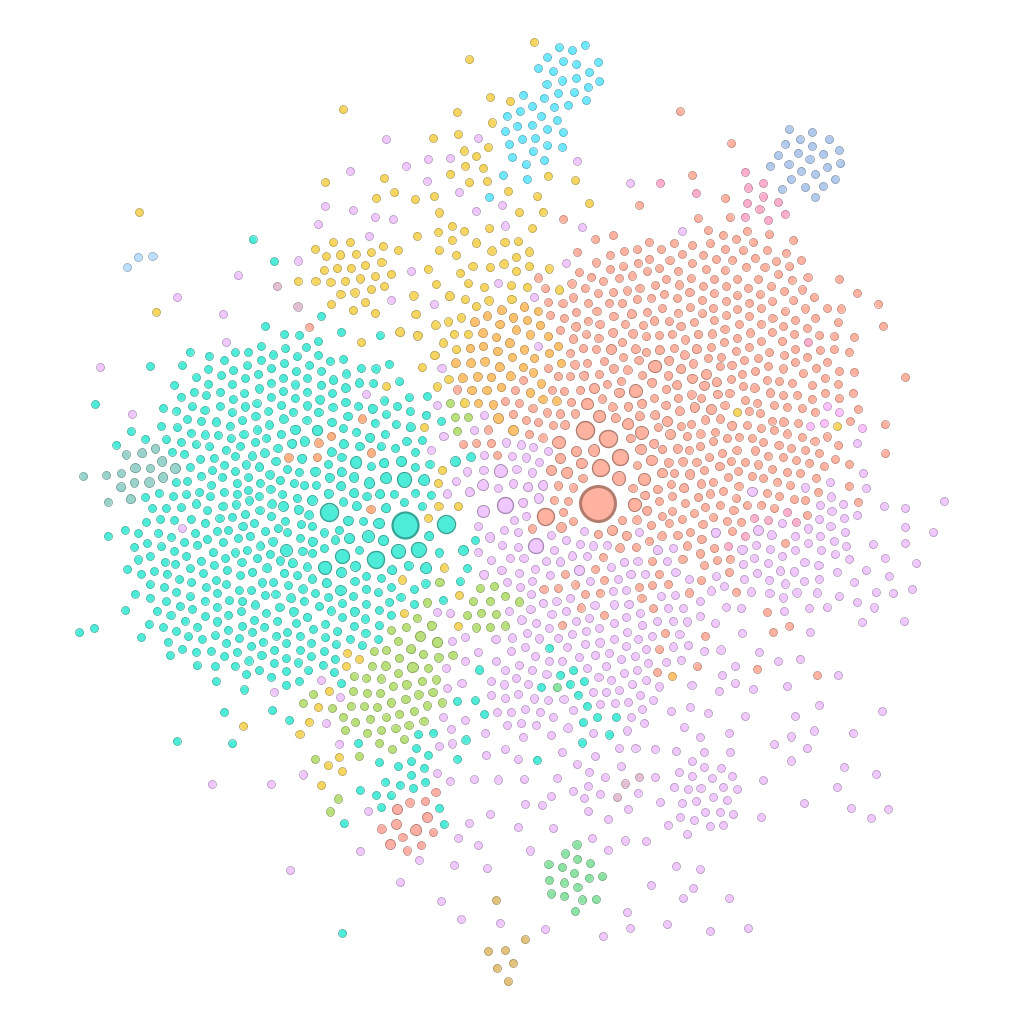
\includegraphics[height=0.5\textheight]{images/net_mod_app}
		\caption{Hashtag network, nodes coloured to modularity class (community) and ForceAtlas 2 layout applied. Notable communities in the network include right-wing terms (red, upper right), left-wing terms (cyan, middle left), "battleground" terms (pink, lower central leaning right), and news-related terms (yellow, upper central leaning left). The size of each node directly correlates to how many times it appears in the data set relative to other hashtags.\hfill}
		\label{fig:1}
	\end{figure}

	\begin{figure}%[hb]
		\centering
		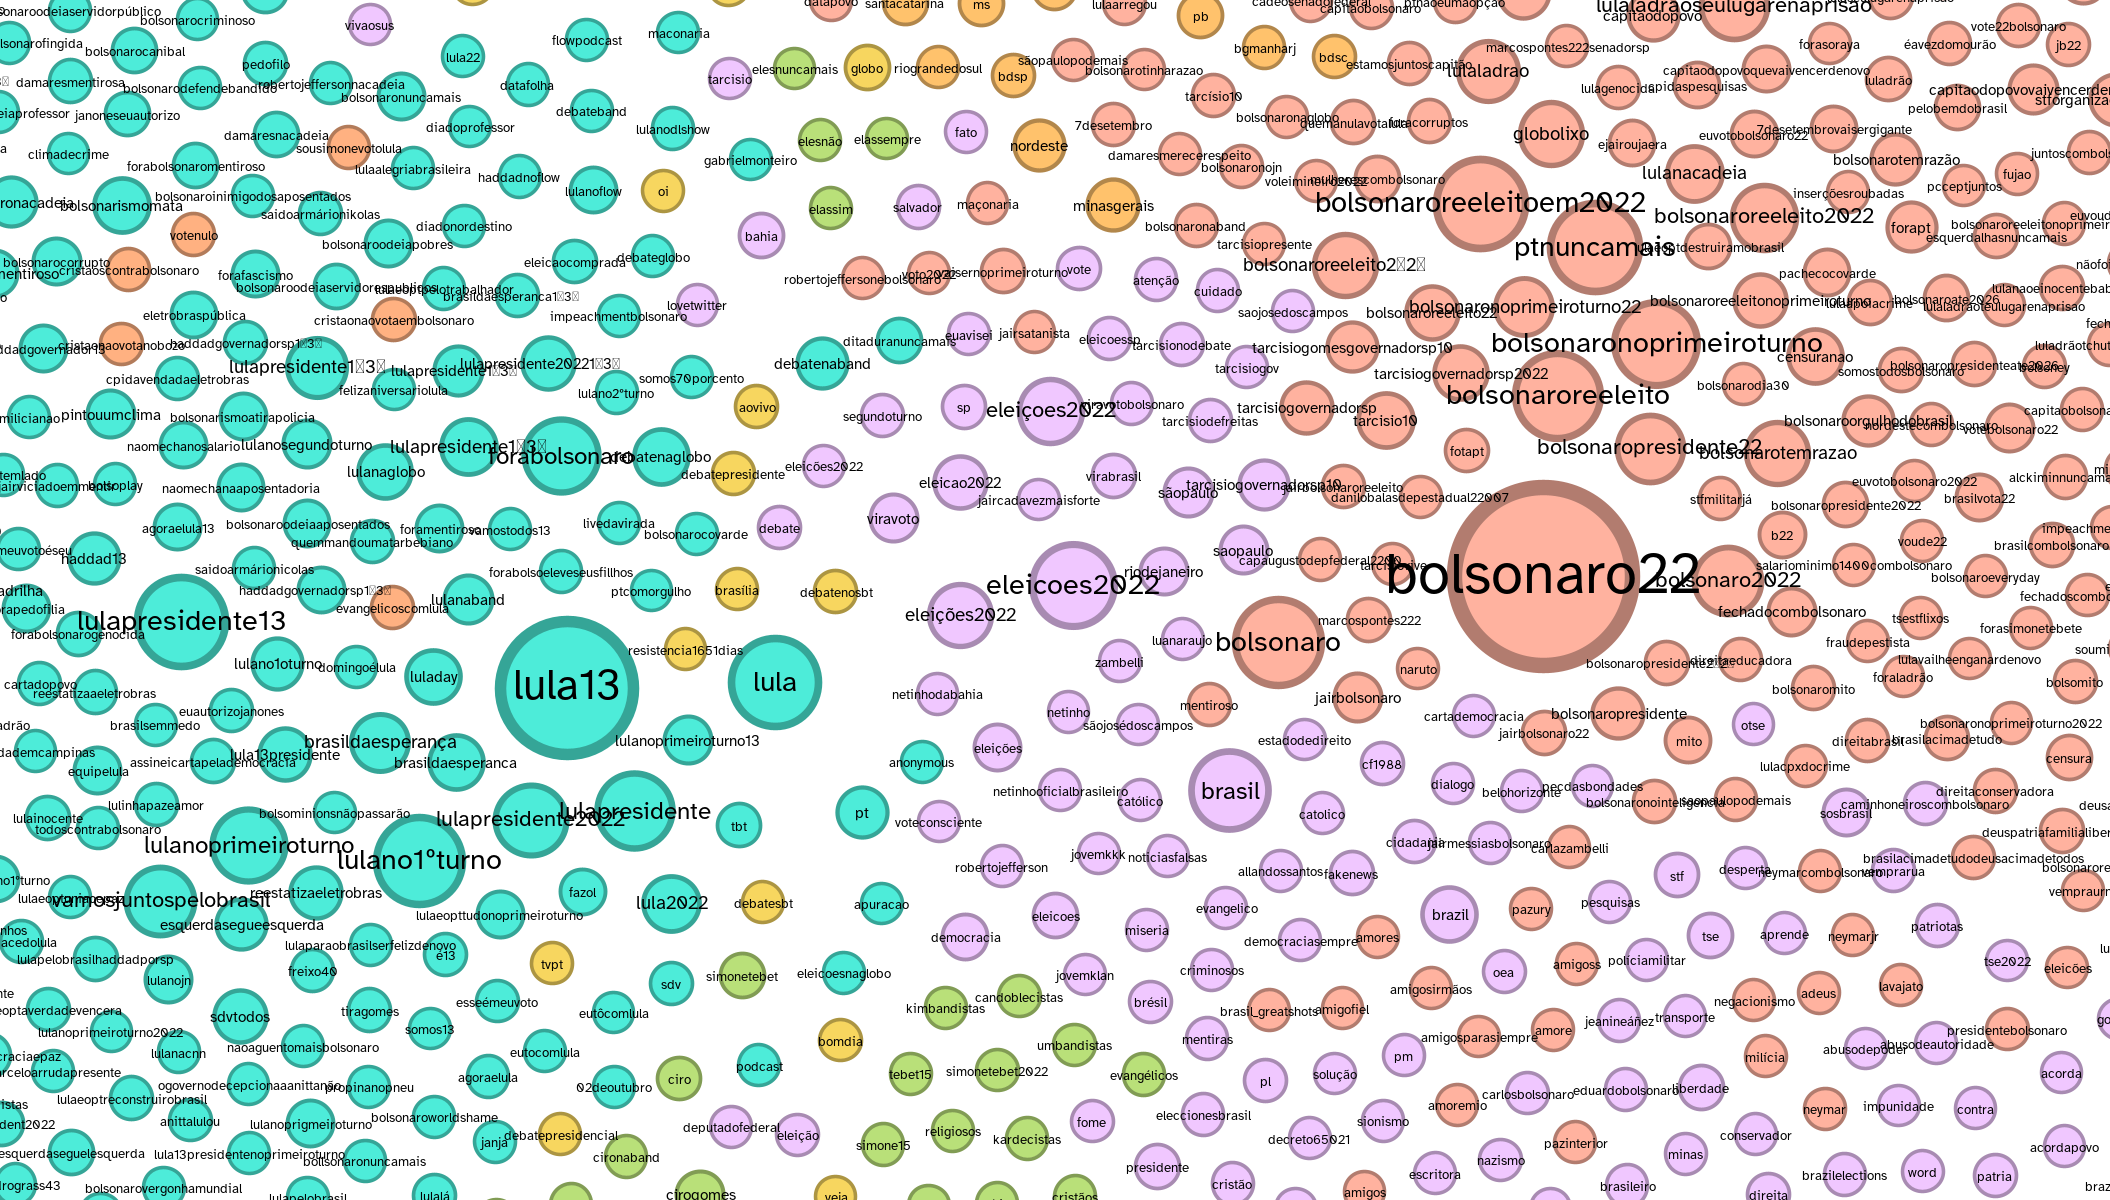
\includegraphics[height=0.3\textheight]{images/net_mod_app_detail}
		\caption{Zoomed view of \autoref{fig:1}'s central region with labels enabled.}
		\label{fig:2}
	\end{figure}

	\autoref{fig:3} shows the same network as in \autoref{fig:1}, but with the node sizes altered to visualise toxicity and bot activity across the network - larger nodes mean a higher likelihood of the hashtag being contained within a toxic post (\autoref{fig:3a}) or having been made by a suspected bot (\autoref{fig:3b}). 
	
	
	\begin{figure}%[h]
		\centering
		\begin{subfigure}[t]{0.48\textwidth}
			\centering
			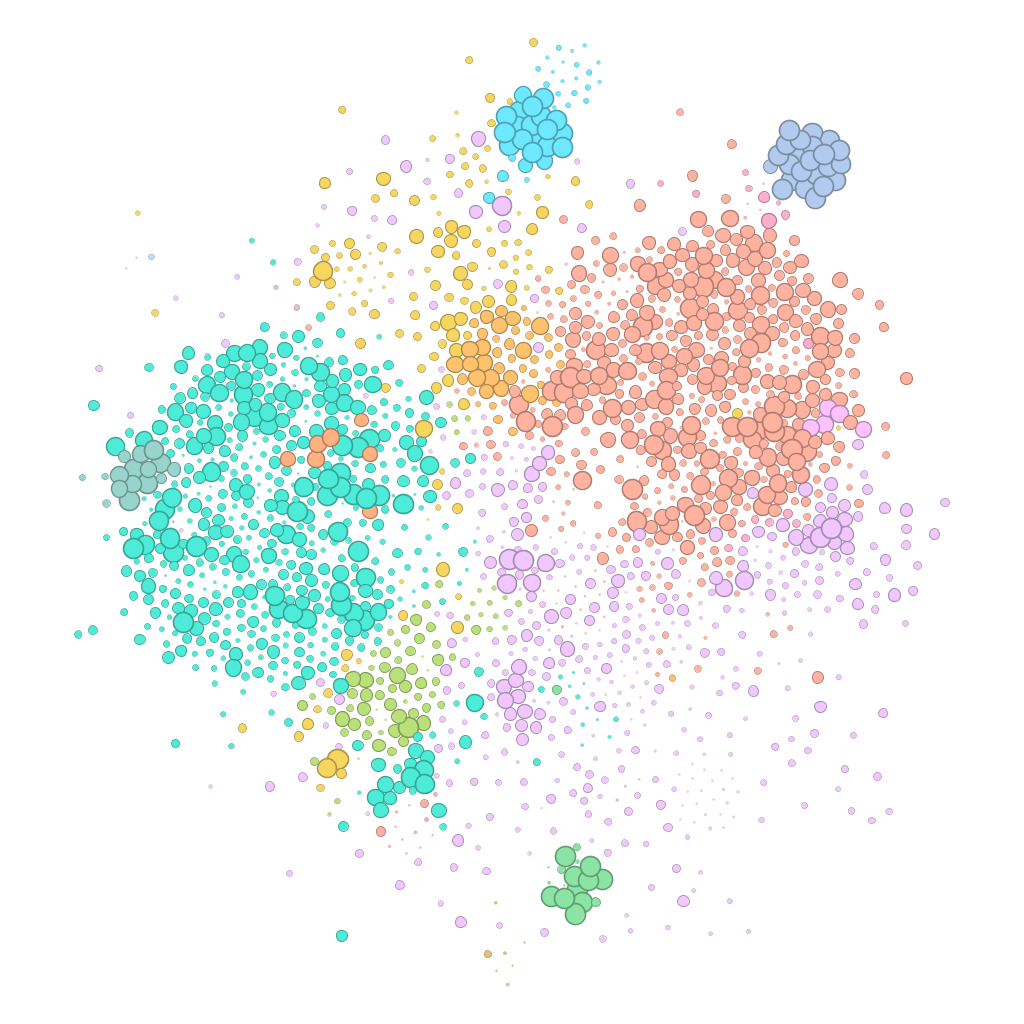
\includegraphics[width=\textwidth]{images/net_mod_tox}
			\caption{\raggedright{Node sizes keyed to average toxicity for posts including hashtag}}
			\label{fig:3a}
		\end{subfigure}
		\begin{subfigure}[t]{0.48\textwidth}
			\centering
			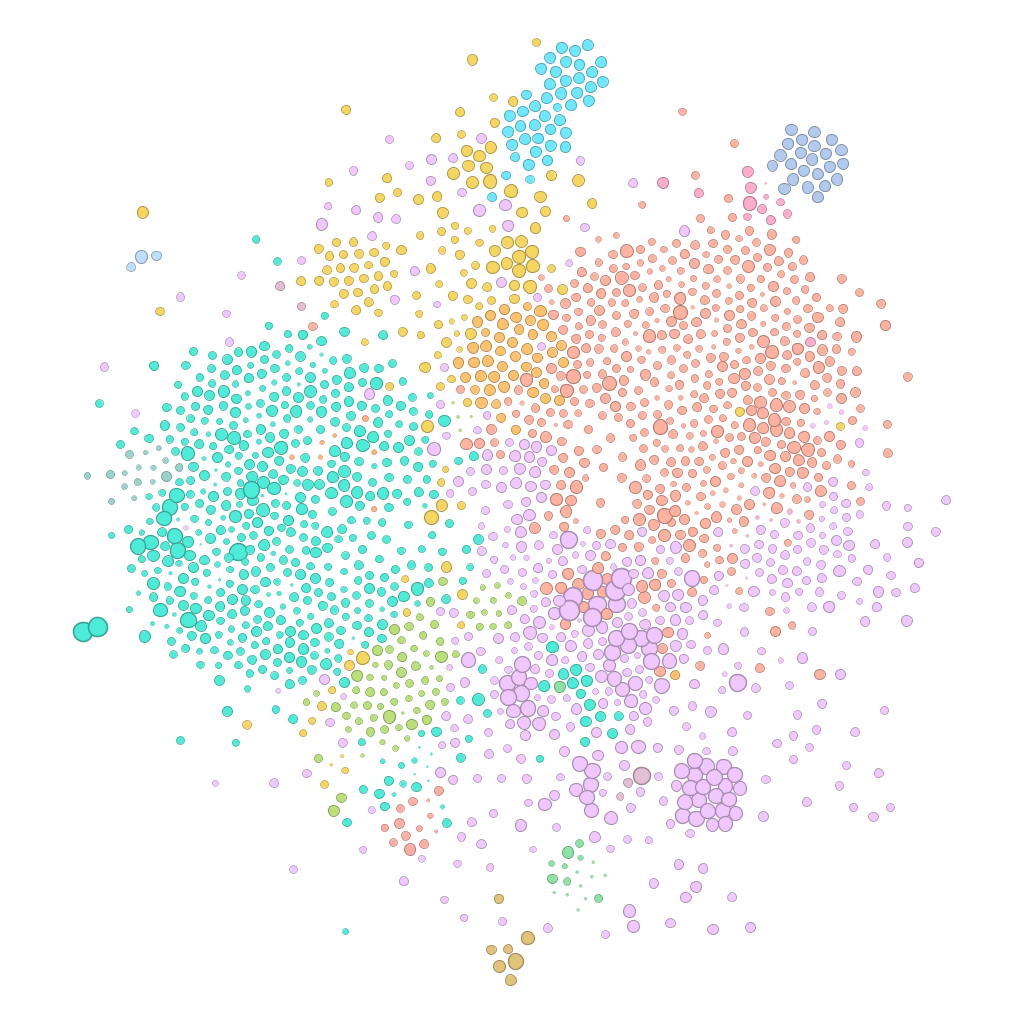
\includegraphics[width=\textwidth]{images/net_mod_bot}
			\caption{\raggedright{Node sizes keyed to average botscore for posts including hashtag}}
			\label{fig:3b}
		\end{subfigure}
		\caption{Hashtag network displaying different size variables, with layout and colouring inherited from \autoref{fig:1}.}
		\label{fig:3}
	\end{figure}

	\begin{table}%[hb]%{L}{9cm}
		\centering
		\begin{tabular}{||l l r||} 
			\hline
			Colour & Topic & \% of network variety \\ [0.5ex] 
			\hline\hline
			Cyan & Left-wing hashtags & 26.7\% \\ 
			\hline
			Red & Right-wing hashtags & 25.8\% \\
			\hline
			Pink & Battleground hashtags & 24.5\% \\
			\hline
			Yellow & News hashtags & 7.2\% \\
			\hline
			Other & All other hashtags & 15.8\% \\
			\hline
		\end{tabular}
		\caption{\autoref{fig:1} and \autoref{fig:2}'s most populous communities. Note that this table only communicates the variety of hashtags, not the quantity of posts made in them.}
		\label{tab:1}
	\end{table}
	
	We can see from a visual inspection that these metrics differ in intriguing ways; toxicity peaks in localised areas of discussion, shown in the many groups of large nodes most visible in the left-wing and right-wing communities separated by gulfs of smaller nodes. Contrastingly, \autoref{fig:3b} implies that nearly all hashtags in our dataset have a base level of bot activity present, with the vast majority of nodes notably larger than the minimum size commonly seen in \autoref{fig:3a}. We can easily confirm this observation, empirically speaking, by comparing the standard deviation of each metric across the whole network. Botscore admits a standard deviation of 0.08, whereas toxicity lies at a much higher 0.22, ratifying our suspicions. We now continue to determine whether this phenomenon may be affected by bots acting as pacifiers and/or agitators.
	
	\subsection{Bots and Toxicity}
	\label{subsec:bottox}
	
	To further explore the data, we simply plot a graph of botscore against toxicity. Sorting all hashtags by their toxicity and calculating an average value, weighted by number of appearances, in a fixed number of regions allows us to directly explore a potential correlation between botscore and toxicity. \autoref{fig:4} shows this graph and informs us of a distinct lack of correlation across the dataset, the mean line largely lying flat. We can, however, see that the vast majority of conversation appears within a densely populated zone between 0.20 and 0.40 toxicity, hovering just below a botscore of 0.30. All together, the shape of the graph somewhat resembles a saddle; this saddle is shown in a pair of faintly drawn parabolas, so as not to distract too heavily from the graph. This effect leaves a deadzone at low botscores in hashtags with moderately high toxicities of 0.40 to 0.60; the implication is that moderately toxic hashtags attract a moderate bot presence. 

	\begin{figure}%[h]
		\begin{center}
			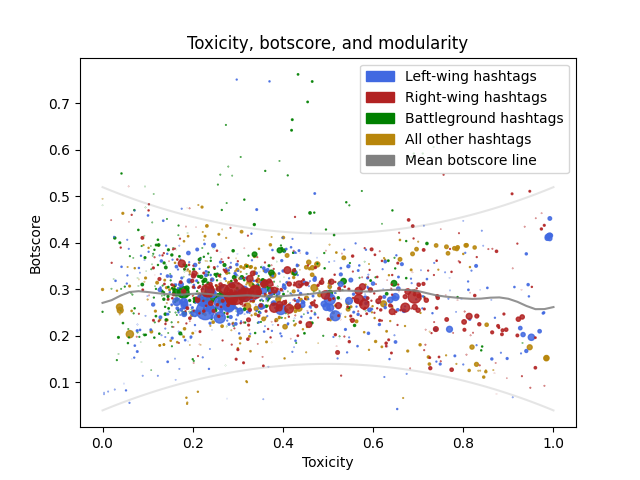
\includegraphics[width=0.9\textwidth]{images/plt_tox_bot_mod}
		\end{center}
		\caption{Scatter graph showing the toxicity and botscore of each hashtag. Sizes of nodes correspond to how many posts included the hashtag (the number of "appearances"), and colours show modularity/community.}
		\label{fig:4}
	\end{figure}

	With this saddle shape in mind, we notice a group of anomalies with notably high botscores at moderate toxicities. These hashtags mostly belong to the "battleground" modularity, with only two from the left-wing modularity. These two are \textit{"13elevoltara"} and \textit{"simboracomlula13"} boasting botscores of 0.75 and 0.74 respectively, meaning \textit{"13 will return"} and \textit{"let's go with lula 13"}. Both of these hashtags are in support of the left-wing presidential candidate Lula da Silva, implying an actor attempted to increase support of the left-wing candidate using bots to amplify their messaging. 
	
	The remaining anomalies are mostly connected to one another in a local network, shown in \autoref{fig:5}. Some refer to regions, such as \textit{"europe"} or \textit{"africa"}, but most of these anomalously high botscore hashtags concern Jair Bolsonaro or "presidential reform". In the context of when the data was collected, Bolsonaro at the time had been in power for 30-36 months and was approaching the end of his term, with our data comprised of discussion surrounding the election which resulted in his defeat by Lula da Silva. As such, notable connections in this network sit between \textit{"nazismo"} (Nazism), \textit{"zionismo"} (Zionism), and two of Bolsonaro's sons' names (Eduardo and Carlos Bolsonaro), both of whom are also involved in Brazilian politics. 
	
	\begin{figure}%{R}{0.5\textwidth}
		\begin{center}
			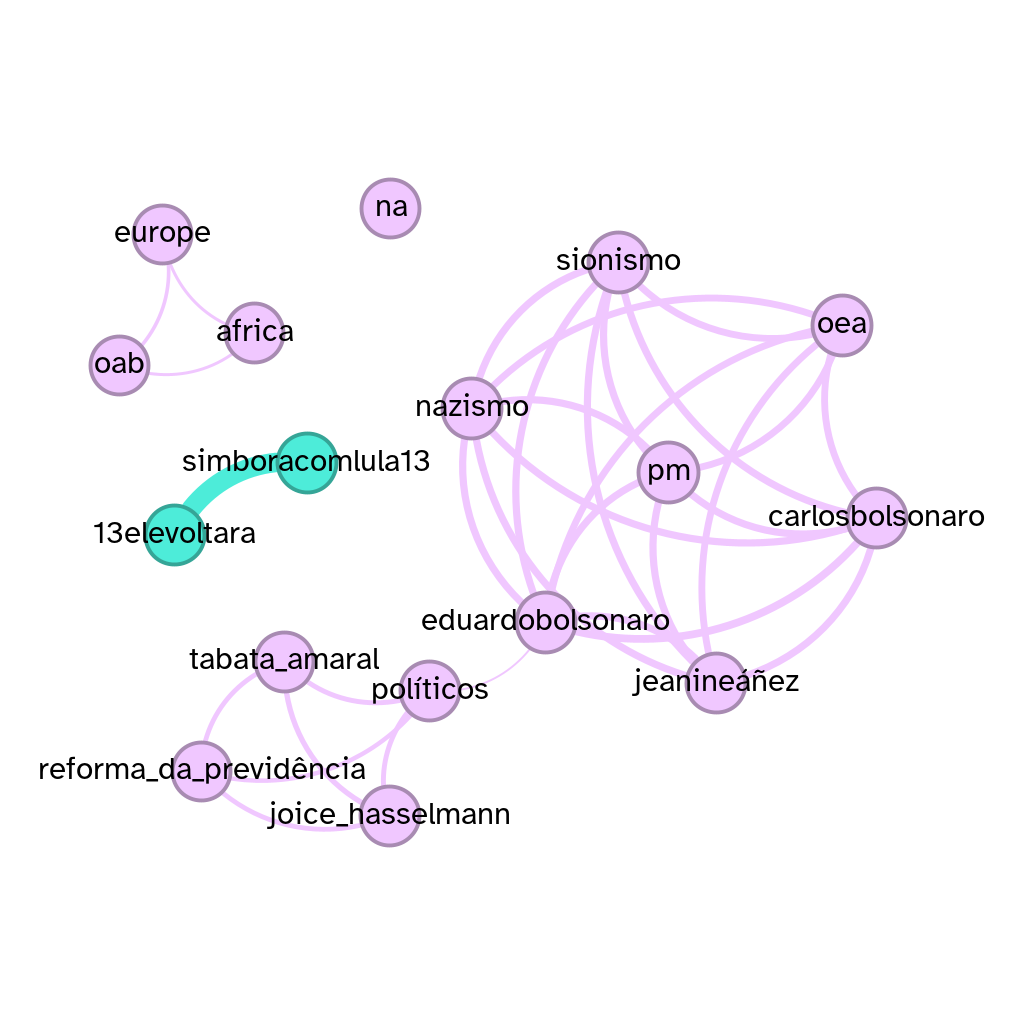
\includegraphics[width=0.6\textwidth]{images/net_anom_detail}
		\end{center}
		\caption{Detail view of the battleground anomalies network.}
		\label{fig:5}
	\end{figure}

	A manual check also reveals that \textit{"nazismo"} and \textit{"zionismo"} both connect to \textit{"bolsonaro"} and \textit{"jairbolsonaro"}, with many of \autoref{fig:5}'s connections appearing exactly 288 times (or within 10\% above 288, never below), shown in the thickness of each edge between nodes. It is fairly likely that these hashtags were levelled as insults against Bolsonaro by a small populace of automated accounts, evidenced by the very high botscore and similar appearance numbers hovering at or just above 288. Many Brazilians dislike Bolsonaro for controversial actions surrounding deforestation of the Amazon rainforest, his handling of the Covid-19 pandemic, and other smaller campaign-related controversies (\parencite{BrazilianAmazonDeforestation}, \parencite{trevisaniBrazilBolsonaroFires2019}, \parencite{dupeyronJustTrumpBrazil2020}, \parencite{BrazilMilitaryChiefs2021}, \parencite{phillipsBrazilJairBolsonaro2018}), though simply existing as a political opponent opens motivation for manipulating opinions as discussed in \autoref{subsec:background}. 
	
	These manipulations may even have been orchestrated by the same actor responsible for amplifying the messaging of \textit{"simboracomlula13"}, using the same techniques to slander Bolsonaro and make him appear a worse fit for the presidential seat. The only reason we have noticed these manipulations is that the botscore of these hashtags appeared notably high, with few "real" people including these hashtags in their discussions; we put forward that similar manipulations are in effect across the dataset, being obscured by the activity of real users. Further, in this case, this anomalous network acts as evidence towards our first hypothesis that bots are being utilised to influence political discussions to become more toxic; hurling insults over the internet is not usually seen as a level-headed gesture.
	
	\subsection{Partitioning by Modularity}

	In this section, we partition the dataset by modularity and perform a similar analysis as in \autoref{subsec:bottox}, but within the two primary communities (left-wing and right-wing) rather than across all processed data. \autoref{fig:6} shows a scatter graph of each major community's points as in \autoref{fig:4} split out to their own graphs with their own mean lines applied. Each mean is calculated as a weighted average, using each hashtag's appearances relative to others as the weighting.
	Each community has its own characteristics shown in the mean line plotted on each graph.
	
	\begin{figure*}%[h]
		\centering
		\begin{subfigure}[b]{0.475\textwidth}
			\centering
			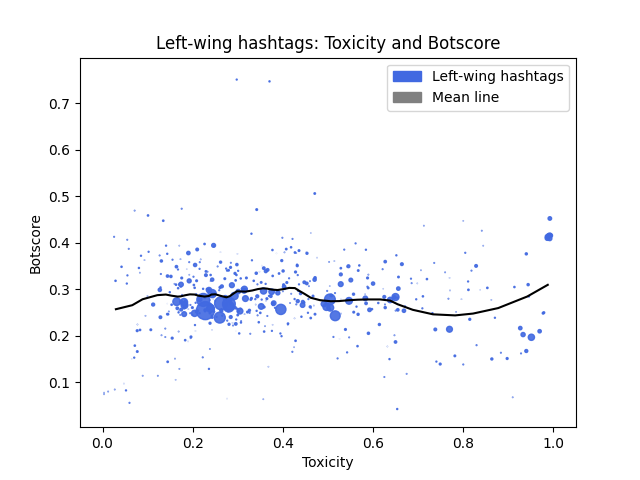
\includegraphics[width=\textwidth]{images/plt_leftwing}
			\caption{Left-wing community scatter graph}
			\label{fig:6a}
		\end{subfigure}
		\hfill
		\begin{subfigure}[b]{0.475\textwidth}  
			\centering 
			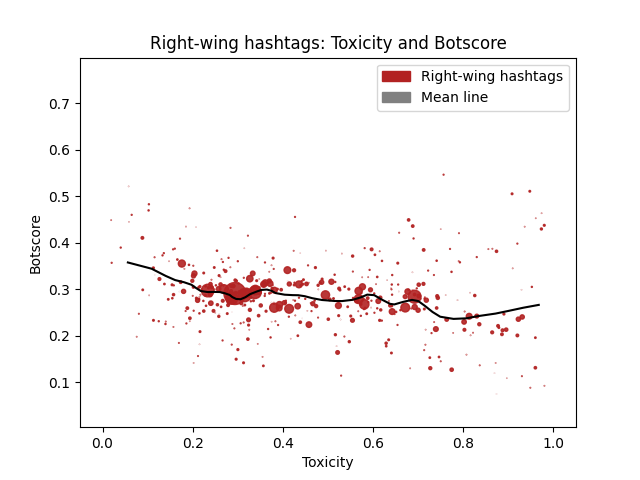
\includegraphics[width=\textwidth]{images/plt_rightwing}
			\caption{Right-wing community scatter graph}
			\label{fig:6b}
		\end{subfigure}
		\vskip\baselineskip
		
		\begin{subfigure}[b]{0.475\textwidth}   
			\centering 
			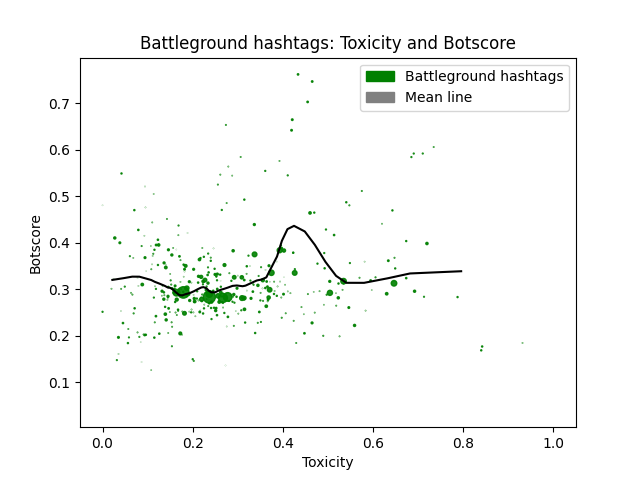
\includegraphics[width=\textwidth]{images/plt_battle}
			\caption{Battleground community scatter graph}
			\label{fig:6c}
		\end{subfigure}
		\hfill
		\begin{subfigure}[b]{0.475\textwidth}   
			\centering 
			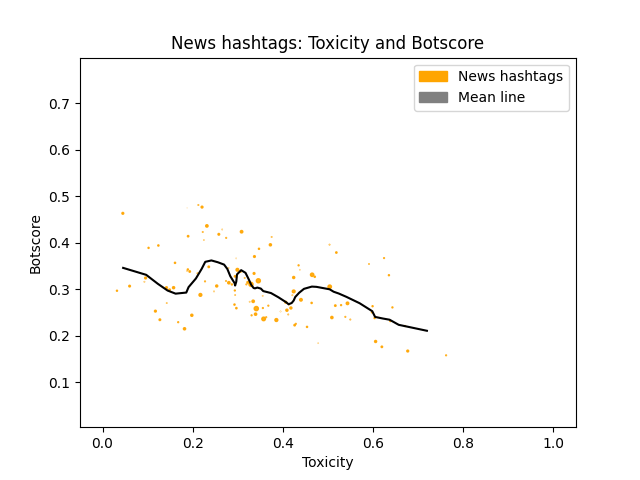
\includegraphics[width=\textwidth]{images/plt_news}
			\caption{News community scatter graph}
			\label{fig:6d}
		\end{subfigure}
		\vskip\baselineskip
		
		\begin{subfigure}[b]{0.475\textwidth}   
			\centering 
			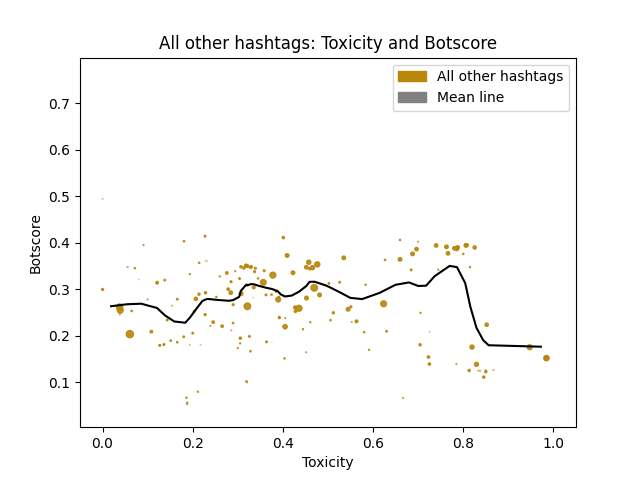
\includegraphics[width=\textwidth]{images/plt_other}
			\caption{All other hashtags scatter graph}
			\label{fig:6e}
		\end{subfigure}
		\hfill
		\begin{subfigure}[b]{0.475\textwidth}   
			\centering 
			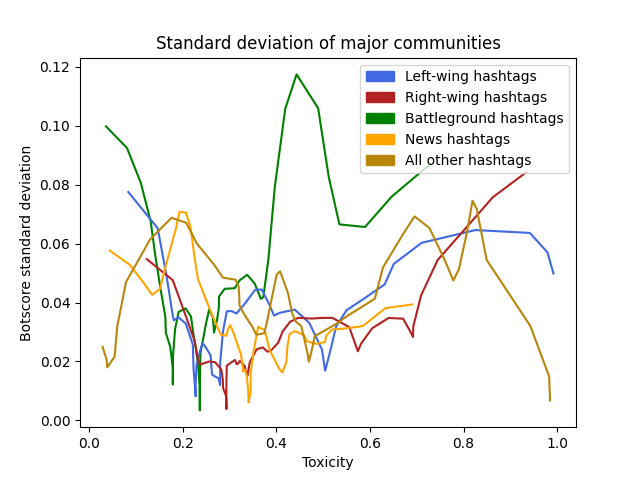
\includegraphics[width=\textwidth]{images/plt_major_dev}
			\caption{Standard deviation of all major communities, weighted to number of appearances}
			\label{fig:6f}
		\end{subfigure}
		
		\caption{Plots of each major community, demonstrating the spread of each community's hashtags along with the local mean weighted for the influence of each hashtag. \autoref{fig:6f} shows the botscore's standard deviation in each community as toxicity varies, accounting again for the influence of each hashtag.}
		\label{fig:6}
	\end{figure*}

	\subsubsection{Left-wing community analysis}

	Left-wing hashtags stay at roughly the same botscore across toxicities, but with a curve upwards at the end likely influenced by the single large hashtag at near-max toxicity. A closer inspection reveals that this is not a single hashtag, but a group of abnormally high botscore hashtags at the highest toxicity values present in the whole dataset. 
	
	This local network is shown in \autoref{fig:7}, and shows how deeply connected these hashtags are. With the size of each node keyed to its appearances, we even notice that all of these hashtags except one boast between 23,000 and 24,000 appearances, the exception having 16,175. Further, many of these connections have weights of exactly 1,753 or 1,754 appearances together, implying that when two of these hashtags were used the others were extremely likely to follow. These close numbers, deeply linked connections, and the high botscore when compared against the rest of the left-wing data together suggest a discussion being deeply influenced by bots. Not only this, but the very high toxicity of these hashtags further suggests these bots may be acting to reinforce a toxic discussion already occurring; at the very least, they aren't helping, otherwise the toxicity of the local network would be lower - the average toxicity of this local network is 0.991, with each hashtag in the top 1\% most toxic in the dataset.
	
	\begin{figure}[h]%{R}{0.5\textwidth}
		\begin{center}
			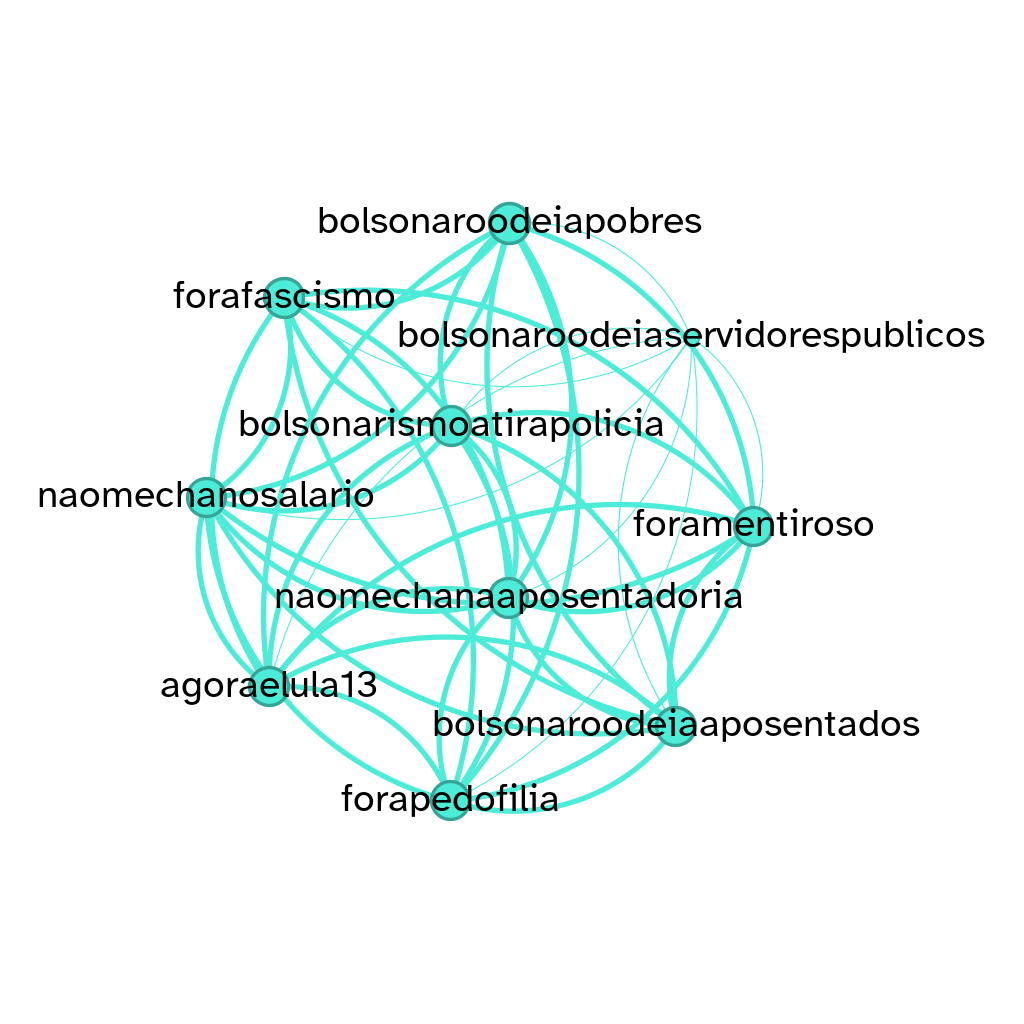
\includegraphics[width=0.6\textwidth]{images/net_leftwing_hightox_highbot}
		\end{center}
		\caption{Detail view of the anomalous high-toxicity high-botscore hashtags in \autoref{fig:6a}.}
		\label{fig:7}
	\end{figure}

	The overall topic of these hashtags lends itself to a toxic discussion. The overall tone is assertive and accusatory, many of these posts likely made during the autumn 2022 presidential election campaigns: \textit{"Bolsonaro hates the poor"}, \textit{"pedophilia out"}, \textit{"fascism out"}, \textit{"don't mess with retirement"}, and \textit{"he was a liar"} are some translated examples from this network. Our earlier observations indicated a discussion highly influenced by bot activity, though these discussion topics and accusations can be expected to begin organically in a modern day election cycle online. Furthermore, the disparity between edge weights and appearances implies these hashtags are often used outside of this deeply linked network in other discussions elsewhere in the network. As such, we can conclude that this is most likely a case of bots being used to amplify a toxic discussion and spread these opinions further rather than bots being utilised to begin one from scratch, potentially leveraging these hashtags to gain a greater reach and influence. These findings further support our hypothesis in \autoref{subsec:bottox} that bot manipulations are easily obscured by the postings of real users, along with reinforcing our earlier suspicion that bots are indeed influencing political discussions to become more toxic.
	
	\subsubsection{Right-wing community analysis}
	In contrast to the flat mean of the left-wing network previously discussed, the right-wing network demonstrates a moderate negative correlation between toxicity and botscore with a slight upturn in botscore at the highest toxicities. On a visual inspection, the right-wing network appears to contain more hashtags at the higher end of the toxicity scale. We can investigate this difference by calculating the mean and median of both botscore and toxicity for each community, shown in \autoref{tab:2}.

	\begin{table}[h]
		\begin{center}
			\begin{tabular}{||l | r | r | r | r||}
				\hline
				Community & \multicolumn{2}{c|}{Toxicity} & \multicolumn{2}{c||}{Botscore} \\ 
				\cline{2-5} 
				& Mean & Median & Mean & Median \\
				\hline \hline
				Left-wing & 0.38 & 0.35 & 0.28 & 0.28 \\ 
				\hline
				Right-wing & 0.43 & 0.42 & 0.29 & 0.29 \\ 
				\hline
				Battleground & 0.28 & 0.25 & 0.31 & 0.30 \\ 
				\hline
				News & 0.35 & 0.33 & 0.30 & 0.30 \\ 
				\hline
				Other & 0.46 & 0.36 & 0.28 & 0.28 \\ 
				\hline
			\end{tabular}
			\caption{\raggedright{Statistics comparison table for all major communities. Means are weighted to appearances.}}
			\label{tab:2}
		\end{center}
	\end{table}

	As suspected, when compared to other focused communities, the right-wing community has a notably higher mean and median toxicity, with mean and median botscores in the expected range. Note in this case that "other" hashtags also have a very high toxicity; this is due to the varied and unfocused discussion occurring across the remaining 14 communities which all in all comprise only 15.8\% of the data's variety (\autoref{tab:1}); furthermore, the right-wing community has a direct counterpart in the left-wing, and as such we continue our inspection of this comparatively high toxicity. While a similar upturn occurs at the high end of toxicity as in the left-wing community, the intensity of the right-wing's equivalent is much lower with a manual inspection revealing many much less popular hashtags appearing to bring this line upwards. With this finding in mind, along with the mean botscore steadily lowering as toxicity increases, we show that these right-wing discussions appear to simply trend towards toxicity without any notable bot influence attempting to coerce the discussion towards it; in fact, these toxic discussions consistently contain less bots the more toxic they become. 
	
	We now check this finding by inspecting the weighted standard deviations of each community across toxicities. \autoref{fig:6f} shows this plot, demonstrating that the right-wing community is overall one of the closest-fitting to the baseline data. However, as toxicity rises we also see the standard deviation rise steadily. This curve shows us that, at the highest toxicities, there is a wide range of hashtags with both high and low botscores active in the community. For this reason, we can say in this case that fringe communities of bots are attempting to influence political discussions on the right to become more toxic. 
	
	The affected hashtags at this highest end of toxicity include \textit{"capitaobolsonaro"}, \textit{"stfmilitarjá"}, \textit{"eleicoessemsacanagem"}, and \textit{"capitaoparaobemdanacao"}, all of which have appearances totalling between 4,000 and 5,000. While not obvious or egregious as the similar anomaly network in the left-wing graph, we can consider this a very similar case of bots amplifying a toxic message. The translated hashtags are \textit{"captain Bolsonaro"}, \textit{"STF military now"}, \textit{"elections without bullshit"}, and \textit{"captain for the good of the country"}, clearly referring to Bolsonaro again. 
	
	\textit{"Elections without bullshit"} is reminiscent of slogans adopted by western alt-right political movements concerning election fraud such as \textit{"stop the steal"}, popularised by the high-profile defeat of Donald Trump in the American 2020 presidential election\parencite{FederalElections2020a} and his following campaign to overturn the result on claims of voter fraud\parencite{rutenberg77DaysTrump2021}, \parencite{ruparTrumpDesperateSTOP2020}, eventually culminating in the attack on the American political centre of the Capitol on January 6th, 2021 \parencite{JanuaryAttackCapitol}, \parencite{JanuaryCapitolAttack2024}. Similarly, \textit{"STF"} refers to the Brazilian Supreme Federal Court\parencite{STJInternationalSuperior}; due to the extremely high toxicity of the hashtag, it's possible these posts were attempting to incite violence against members of the court or prompt the STF to "use" the military in some degree, a line of thinking potentially borrowed once again from Trump and his supporters' militarisation \parencite{lohStopStealLeader},\parencite{sonmezFrustratedTrumpRedoubles2020}. As further evidence, \textit{"captain Bolsonaro"} and \textit{"captain for the good of the country"} appear to idolise Bolsonaro, depicting him almost as a military leader guiding the populace towards a better future.
	
	With the botscores and topics of these most common toxic right-wing hashtags in mind, we can conclude once again that communities of bots are attempting to amplify incendiary ideas and topics across the wider spectrum of discussion.
	
	\subsection{Frequency Analysis}
	We conclude our analysis with a deeper look into the frequency of hashtags used across time. \autoref{fig:8} depicts the graph of posts made over time in the data, while \autoref{fig:9} takes a more focused approach into each major community. At a basic inspection of \autoref{fig:8}, we see quickly that the month of October 2022 sees greatly inflated posting numbers correlating to the presidential election on 2 October 2022, concluding in the runoff election on 30 October 2022 deciding the presidential winner after the 2 October election failed to determine a winning candidate with more than 50\% of votes. After these events, activity sharply drops to pre-election levels. The smaller spikes in August correspond to the beginning of the election cycle on 16 August 2022, with the first presidential debate taking place on the 28th of the same month.
	
	\begin{figure}%[h]%{R}{0.5\textwidth}
		\begin{center}
			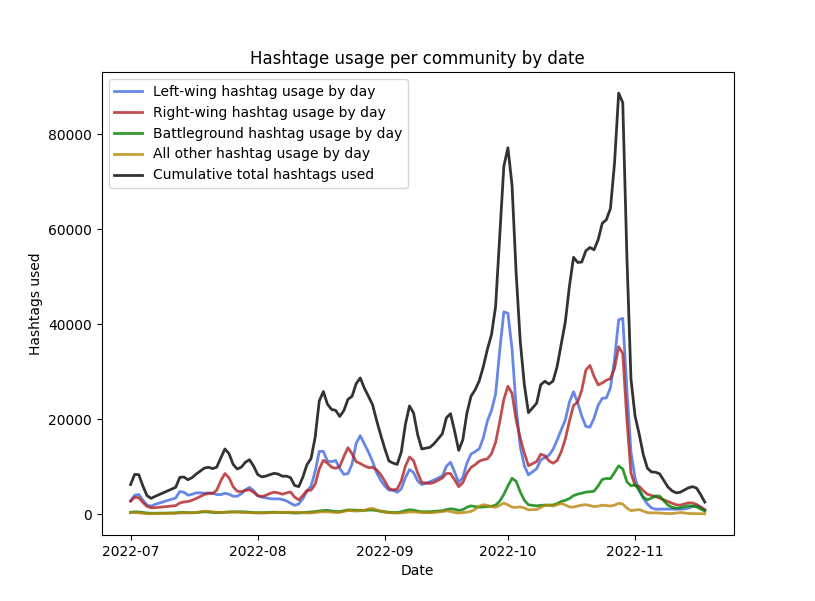
\includegraphics[width=0.8\textwidth]{images/plt_major_appearances}
		\end{center}
		\caption{Graph of cumulative-by-day hashtag frequency over time. Note the spikes at the beginning and end of October coinciding with the dates of the presidential election (2 October 2022) and the secondary runoff election (30 October 2022) used to break the tie of the first.}
		\label{fig:8}
	\end{figure}
	
	From \autoref{fig:9}, we can determine that botscore stays relatively constant across all postings over time in all communities, with small spikes present mostly in the battleground community. Taken alongside the data shown in \autoref{fig:8}, we can notice that the quantity of posts vastly increases while the mean botscore stays relatively stable. In order for this to be true, bots must be posting content at a proportional rate to the overall frequency of discussion. This insight allows us to further interrogate the motivations of those running these bots; clearly, increasing their combined rate of posting during important election events is not a coincidence, and in fact acts as further evidence for the meddling of automated accounts in these discussions. 

	\begin{figure*}%[h]%{R}{0.5\textwidth}
		\begin{center}
			\makebox[\textwidth]{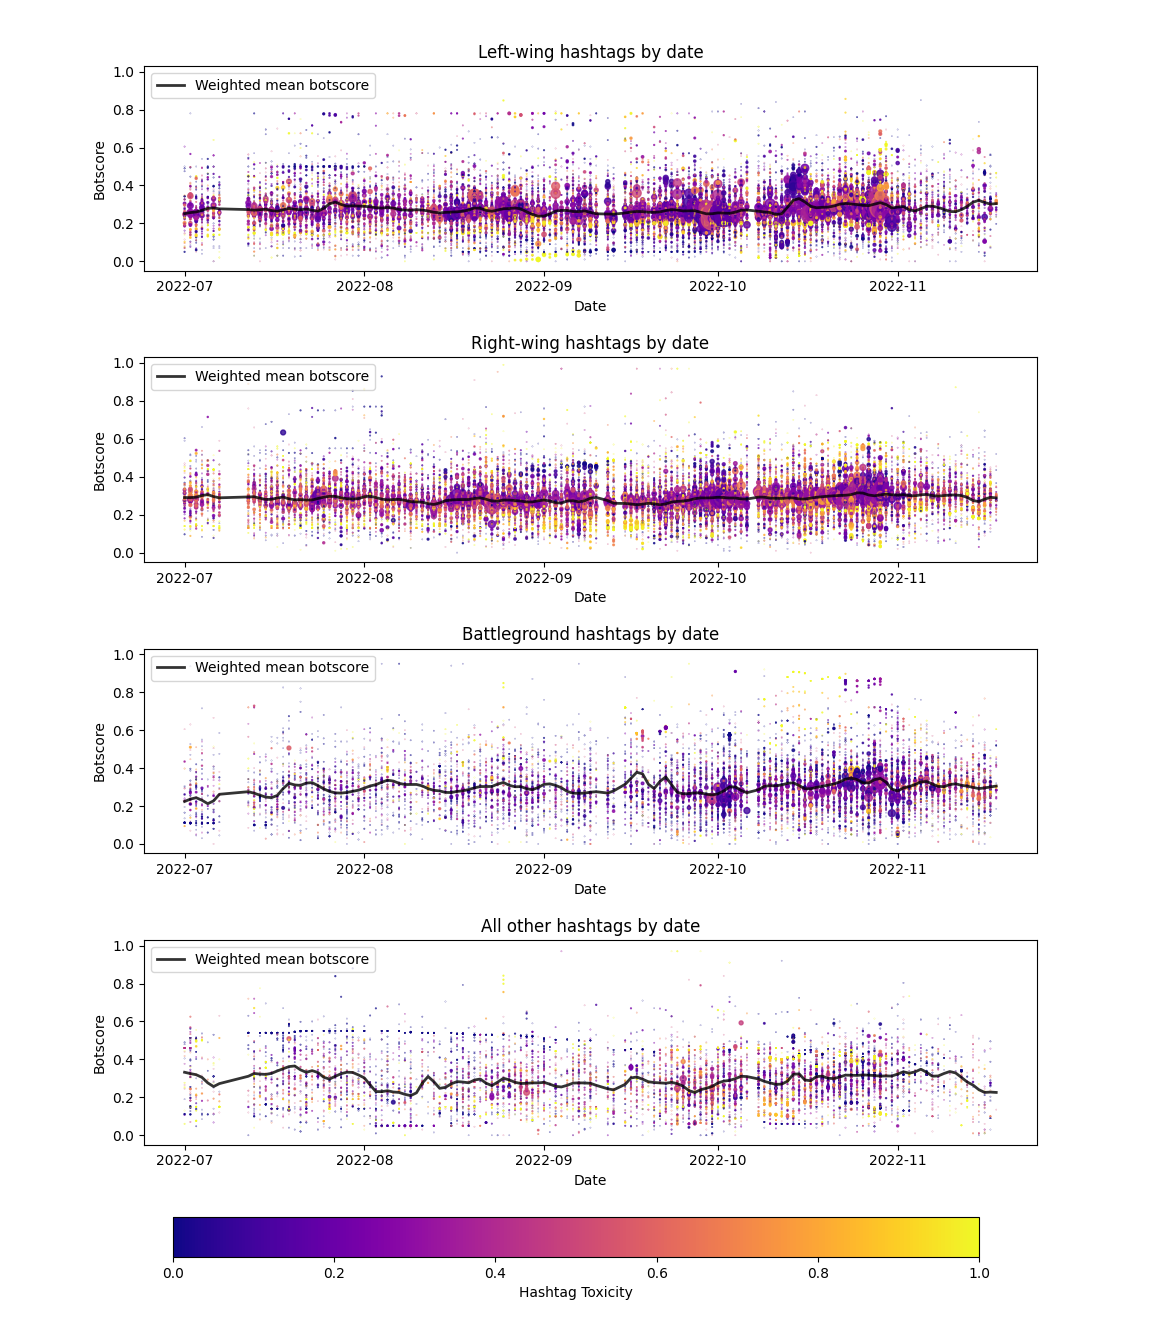
\includegraphics[width=1\paperwidth]{images/plt_major_bydate}}
		\end{center}
		\caption{Graphs of botscore against date within each community, with the colouring of nodes depicting toxicity. Botscore means are calculated as a weighted average.}
		\label{fig:9}
	\end{figure*}\textbf{}
	
	Inspecting this data with an eye towards toxicity we notice that, while the right-wing community has been shown to be more toxic overall (\autoref{tab:2}), the left-wing appears to become more toxic - and more affected by bots - around election dates, shown in the left-wing section of \autoref{fig:9} in the days leading up to 30 October 2022. This effect does not appear to be present in the right-wing community, nor any of the others. While the battleground community does have a few suspiciously high botscores around these elections, the overall toxicity of the community appears to be low consistently through the entire election cycle. The disparity between these two primary communities of left-wing and right-wing discussion yet again provides evidence towards our claim that bots are interfering with political discussions to become more toxic, but with a caveat: these bots appear to be picking and choosing, leaving right-wing discussions mostly alone while attempting to more deeply influence left-wing discussions to become more inflammatory. To further confirm this, we inspect the high-toxicity high-botscore hashtags posted on 30 October 2022 - the runoff election date.
	
	Examples of these suspect hashtags include \textit{"lulapresidente2022"}, \textit{"bolsonarismomata"}, \textit{"forabolsonaro"}, and \textit{"bolsonaropedofilo"}, respectively translating to \textit{"President Lula 2022"}, \textit{"Bolsonarism kills"}, \textit{"Bolsonaro out"}, and \textit{"paedophile Bolsonaro"}. Further, we also find once again every single one of the hashtags shown in \autoref{fig:7}.  We can clearly see that many of these hashtags naturally lend themselves to a toxic discussion; boosting their reach and influence with bots serves to increase toxicity while simultaneously supporting Lula da Silva by slandering\footnote{Jair Bolsonaro to our knowledge has not been convicted of paedophilia, though he once did say he "felt a spark" with "14 and 15-year-old girls" in mid-October of 2022\parencite{BolsonaroSaysHe2022}. This is likely where the popularity of \textit{"bolsonaropedofilo"} in our data originates.} of the opposing candidate. The exception to these topics is \textit{"lulapresidente2022"}, a seemingly innocent hashtag with a notably high botscore and toxicity of 0.41 and 0.69 respectively in this day. In this case we theorise that due to the high popularity of the hashtag, an attempt by another group to perform a \textit{"hashjack"} may have been performed by coordinated bots to undermine left-wing discussion on the election day. A "hashjack" is a coordinated effort to stifle or otherwise repurpose an established discussion for another purpose, most commonly undertaken by alt-right groups \parencite{dariusHowFarRightPolarises2022}.
	
	\section{Limitations and Further Work}
	\subsection{Computation time}
	\label{subsec:computation}
	The primary problem encountered during this project was the scale of computation required for a satisfactory analysis. The largest computation was by far the requirement of running the toxicity prediction model, ToLD-Br\parencite{leiteToxicLanguageDetection2020}, on just under 1 million unique texts.
	
	The strain of running this toxicity prediction model is the primary reason for the aggressive nature of our data filtering. Each text prediction took on average 0.2 seconds to perform on the available computing power (see \autoref{app:work}) - the dataset as a whole contains 437 million posts. This quantity of data is beyond enormous, and processing all of it is clearly unfeasible for the time allocated to the project\footnote{For completeness, this calculation would take an estimated 3 years (\texttt{0.2 * 437,000,000} seconds) on the hardware available.}.

	The filters applied, in order, are as follows:
	\begin{enumerate}
		\item Full dataset, August 2018 to March 2023 (approx. 437 million posts)
		\item Recent data after collection term adjustment, July 2022 to March 2023 (80,688,513 posts)
		\item Only posts containing hashtags (7,806,357 posts)
		\item Removed all reposts (3,523,010 posts)
		\item Only posts which contain a hashtag either:
		\begin{itemize}
			\item directly appearing in the modularity class related to left-wing or right-wing posts (\autoref{subsec:modularity}),
			\item appearing alongside one of the previous hashtags (968,627 posts)
		\end{itemize}
	\end{enumerate}
	Implicit in step 5 of this filtering is the fact that the hashtags are extracted "backwards" from posts which appear more than 999 times in the data collected in step 2; a small number of posts only containing these "rare" hashtags will have also been removed from the search in this step.
	
	These 968,627 posts were then taken as the final set of posts to be processed through ToLD-Br. Multiplying the expected time of 0.2s each with the 968,627 posts to process, the processing of the data was predicted to take approximately 54 machine hours. Due to bugfixes and memory-full errors causing unexpected crashes, this process took just under 6 days to complete.
	
	If we had not performed the extra pruning in step 5, we would have run the toxicity model for step 4's 3,523,010 total texts. Due to the nature of the data, removing texts not directly linked to the primary modularities for processing would be unlikely to greatly affect conclusions; pruned texts would by definition be unrelated to the primary analysis target of partisan discourse, and so a 73\% reduction in expected computation time was accepted as a worthwhile trade.

	\subsection{Sentiment and stance analysis}
	\label{subsec:sentiment}
	At the same time as the toxicity analysis was performed (\autoref{subsec:toxicity}), a sentiment analysis was also attempted on the final set of filtered posts. Our sentiment analysis corpus was SentiLex-PT02, a well-respected corpus for Portuguese specialised towards "opinions targeting human entities"\parencite{carvalhoSentiLexPT021970}; a corpus in this sense is effectively a lookup table allowing us to correlate words to opinions. SentiLex-PT02 is provided under the Creative Commons Attribution (CC-BY) license, and required some modifications before it was appropriate for our usage.

	The final sentiment analysis algorithm iterated through the following steps:
	\begin{enumerate}
		\item Preprocess the original text of each collected post through a standard natural language processing pipeline (tokenisation, lowercasing, removal of punctuation and stopwords, stemming)
		\item Iterate over each word in the text and check for its existence in the sentiment analysis corpus
		\item If the item does not appear, move to the next word. If it does, determine the word's polarity ($+1$ or $-1$)
		\item Add the polarity to a tracker variable, beginning at 0
		\item For each hashtag, collect all posts containing that hashtag and calculate the mean sentiment of the posts. 
		\item Normalise each result between 0 and 1, 1 being "positive" and 0 being "negative"
	\end{enumerate}
	This approach yielded results that were considered near-useless, despite our best understanding of how to tackle the problem. Extreme outliers and many "neutral"\footnote{It is possible that some texts contained equal amounts of positive and negative polarity words, resulting in a neutral assessment.} texts contained in the data meant the vast majority of hashtags held a sentiment value between 0.48 and 0.52, very close to the neutral value of 0.5.

	The purpose for the development of this sentiment analysis algorithm was to support the further development of a stance analysis algorithm. A stance analysis is a form of opinion classification with the goal of using a text to interpret the author's true feelings towards the target (subject).
	\textcite{aldayelStanceDetectionSocial2021} concisely demonstrates the delineation between sentiment and stance in \autoref{tab:3}, alongside the quote found under the table.

	\begin{table}[htb!]
	% DO NOT TOUCH RENDERS PERFECTLY
		\caption{Table 1 verbatim from \citeauthor{aldayelStanceDetectionSocial2021}, showing the sentiment polarity of the expressed stance. Note that positive or negative stances can have positive, negative, or neutral sentiments.}
		\label{tab:3}
		\begin{center}
			\begin{tabular}{||l p{0.52\linewidth} p{0.16\linewidth} l l||} 
				\hline
				\# & Tweet & Target & Sent. & Stance \\ [0.5ex] 
				\hline\hline
				1 & \raggedright{It is so much fun having younger friends who are expecting babies.} \#beentheredonethat \#chooselife & Legalisation of abortion & + & - \\ 
				\hline
				2 & \raggedright{Life is sacred on all levels. Abortion does not compute with my philosophy.} (Red on \#OITNB) & Legalisation of abortion & 0 & - \\ 
				\hline
				3 & \raggedright{The biggest terror threat in the World is climate change \#drought \#floods} & Climate change is a real concern & - & + \\ 
				\hline
				4 & \raggedright{I am sad that Hillary lost this presidential race} & Hillary Clinton & - & + \\ 
				\hline
			\end{tabular}
			\vspace{0.2cm}
			\begin{quote}
				"...several studies have demonstrated that it is insufficient to use sentiment as the only dependent factor to interpret a user’s stance (Aldayel and Magdy, 2019b; Elfardy and Diab, 2016; Mohammad et al., 2017; Sobhani et al., 2016; Somasundaran and Wiebe, 2009). This is due to the complexity of interpreting stances from a given text, as they are not always directly aligned with the polarity of a given post."
				\attrib{\citeauthor{aldayelStanceDetectionSocial2021}, \citeyear{aldayelStanceDetectionSocial2021}}
			\end{quote}
		\end{center}

	\end{table}
	
	In the interest of overall project success and with the knowledge that the toxicity and botscore analyses were producing appropriate results (i.e. behaving correctly), the work to correct the sentiment analysis engine was abandoned as it would only support the following creation of a stance analysis engine; all in all, a much larger undertaking. While the success of this algorithm and the following results surely would have allowed a more nuanced inspection of the data (and the exploration of the original secondary question shown in \autoref{subsec:spec}), the results found from the toxicity and botscore analyses (\autoref{sec:results}) stand on their own and should be considered complete in themselves.
	
	The further development of a functioning sentiment and stance analysis can be considered as a high-priority potential extension to our work, and its application a ripe area for further research in this dataset.

	\subsection{"Self-selection" bias}
	\label{subsec:bias}
	There is a notable potential error in that by filtering to only posts containing hashtags, we are not fully considering the landscape of discussion. As seen in \autoref{subsec:computation}, approximately 10\% of the dataset contains hashtags; what of the other 90\%? Could it be possible that bots are more or less likely to include hashtags in their postings at a baseline, and does that mean the overall discourse is differently prone to bot manipulation than we have found? 
	
	Finding empirical answers to these questions is out of the scope of this work, leaving our conclusions vulnerable to this issue, but does provide an exciting opportunity for further research in the field. With this in mind, the findings presented here should be understood with the caveat that the final analysis is purposely limited to posts including hashtags in order to accommodate the earlier modularity analysis (\autoref{subsec:modularity}); the work does not prove or disprove any conjecture in particular because of this limitation, but does provide obvious pathways for investigation in order to more concretely verify these findings by developing methods to expand the community detection beyond hashtag collocations and perform a similar analysis, ideally on an even larger dataset by the use of a more powerful computer.

	\section{Conclusion}
	\label{sec:conclusion}
	The original aim of this project was to investigate possible correlations between toxicity, botscore, and community in online political discussion specifically taking place on the microblogging site X, formerly Twitter. In the course of this investigation, we identified multiple times evidence of bots being leveraged to increase the toxicity of political discussion, especially in left-wing spaces. We would consider this to answer our first original question put forward in \autoref{subsec:spec}, and as such we would consider the project as a success under its own criteria. Not only this, but our findings in \autoref{tab:1} of a heightened toxicity overall in the right-wing community - along with bots acting specifically to increase toxicit in the left-wing - provide a strong baseline for our second revised question to be more deeply considered. The manipulation of communities to trend towards toxic speech is, through these findings, a real concern warranting a deeper investigation.

	To provide some examples of further questions raised by our work which could be undertaken as individual projects in future:
	\begin{enumerate}
		\item What topics do bots tend to prefer speaking about?
		\item Why do toxic bots appear to favour left-wing spaces for targeting?
		\item Is there an underlying reason for the negative correlation between toxicity and botscore in right-wing communities as shown in \autoref{fig:6b}?
		\item Are these bots acting as coordinated groups, or do they seem to act alone? If they work in groups, how large are these groups? Do multiple groups appear to be working towards a shared goal?
		\item Do bots acting in a political community tend to agree or disagree with their community? Does this change in different communities?
		\item Do the same bots often work across communities, or do they mostly remain stationary in a given community?
	\end{enumerate}
	
	Future analyses and investigations are advised to approach the task in a more granular way, investigating more closely specific networks of bot postings and their content such that they might find a more concrete answer to our revised second question, also put forward in \autoref{subsec:spec}. We advise these future works to familiarise themselves further with Pacheco's previous work, especially \textcite{pachecoUncoveringCoordinatedNetworks2021}, to assist them in identifying these coordinated communities. Further, the successful development of a sentiment and stance analysis engine would certainly support this fine-grain community analysis in determining the intent and aims of those coordinating the actions of bots in political spaces; this is, in our opinion, the most important direction for future research in this area.
	
	\newpage
	\begin{appendices}
	\section{Workstation}
	\label{app:work}
	All computation for this dissertation was performed using the author's personal machine on a Linux/GNU installation dedicated specifically for the task. The machine's relevant specifications are as follows:
	\begin{itemize}
		\item CPU: AMD Ryzen 5 5600G (3.7GHz, 4.6GHz boost)
		\item GPU: NVIDIA RTX 2070 SUPER (2560 CUDA cores, 8GB VRAM)
		\item RAM: 16GB Corsair "Vengeance" (3200MHz)
		\item OS: Linux Mint 21.3 "Victoria", kernel version 5.15.0
	\end{itemize}
	These specifications were sufficient for the computations being performed, but given a more powerful computer it is possible that the analysis could have been deepened. All data was stored on a high quality NVME M.2 solid-state drive connected directly to the motherboard.
	
	It is possible that with more foresight, access could have been gained to a more powerful device such as Exeter University's ISCA supercomputer. However, it is our belief that by the time we realised this level of computation power would be useful, it would take longer to gain access and learn to use ISCA's systems than it would to simply run the calculations locally.
	\section{Modularity classes}
	\label{app:modularities}
	This appendix contains the full list of modularity classes discovered by the Louvain analysis and the author's best interpretation of what each community represents. Note that the actual modularity class value is arbitrary and assigned during the Louvain analysis.
	
	\begin{center}
		\begin{tabular}{||l l l r||} 
			\hline
			Class & Colour & Topic & \% of network variety \\ [0.5ex] 
			\hline\hline
			7 & Cyan & Left-wing hashtags & 26.7\% \\ 
			\hline
			9 & Red & Right-wing hashtags & 25.8\% \\
			\hline
			1 & Lilac & Battleground hashtags & 24.5\% \\
			\hline
			14 & Yellow & News hashtags & 7.2\% \\
			\hline
			3 & Green &  & 4.2\% \\
			\hline
			0 & Orange &  & 2.4\% \\
			\hline
			16 & Light blue &  & 2.3\% \\
			\hline
			12 & Pink &  & 1.2\% \\
			\hline
			13 & Light green &  & 1.2\% \\
			\hline
			17 & Slightly darker than light blue &  & 1.2\% \\
			\hline
			2 & Aqua &  & 0.8\% \\
			\hline
			5 & Salmon &  & 0.8\% \\
			\hline
			6 & Tan &  & 0.6\% \\
			\hline
			15 & Dark orange &  & 0.4\% \\
			\hline
			4 & Dusty purple &  & 0.3\% \\
			\hline
			8 & Light pink &  & 0.3\% \\
			\hline
			11 & Grey &  & 0.3\% \\
			\hline
			10 & Lighter blue &  & 0.2\% \\
			\hline
		\end{tabular}
	\end{center}
	
	\section{Graph theory vocabulary}
	\label{app:networks}
	This section concerns an explanation of basic graph theory terms as they relate to our project for those unfamiliar with the concepts. Graph theory is a field of mathematics concerning objects (nodes) which define relations to one another by the connections between them (edges). Various algorithms can be used to depict and analyse graphs, making them extremely useful in both visualisation and research.
	
	A node is a discrete point contained within a graph, usually represented as a circle. Nodes can have arbitrary information attached to them for later analysis, such as their names. In our project, individual hashtags are represented as nodes, and we record the number of times each hashtag appears in total. Each node also contains its own toxicity and botscore (\autoref{subsec:toxicity}, \autoref{subsec:botscore}). After the modularity analysis (\autoref{subsec:modularity}), we also record the modularity class each node belongs to.
	
	An edge is a connection between two nodes, usually represented as a line between two nodes. In graph theory, edges can have a direction, but our project has no need for this; as such, our network is "undirected" and simpler overall. Edge weights in our project represent a collocation between a pair of hashtags (\autoref{subsec:collocation}). Like nodes, edges can have arbitrary information attached to them, though the concept of an "edge weight" is very common. A weight represents the importance of an edge; for us, the number of times a collocation appears is a perfect consideration to use as an edge weight. An example of a use for edge weightings is in layout algorithms for network visualisation, demonstrated in our own project in \autoref{fig:1}. The strength of connections between nodes directly influences the layout of the final graph. Modularity analysis as used in \autoref{subsec:modularity} also uses edge weights to determine where community boundaries lie, and which hashtags are contained within each.
	
	\end{appendices}
	%=========================================================================================================
	% Content ends here
	%=========================================================================================================
	
	\newpage
	\label{sec:references}
	\printbibliography
	
\end{document}